\chapter{گراف‌های جهت‌دار}

در این فصل، روی دو دسته از گراف‌های جهت‌دار تمرکز می‌کنیم:
\begin{itemize}
\item \key{گراف‌های بدون دور}:
هیچ دوری در گراف وجود ندارد،
بنابراین هیچ مسیری از هیچ گرهی به خودش وجود ندارد\footnote{گراف‌های جهت‌دار بدون دور گاهی DAG نامیده می‌شوند.}.
\item \key{گراف‌های جانشین}:
درجه خروجی هر گره ۱ است،
بنابراین هر گره یک جانشین یکتا دارد.
\end{itemize}
مشخص می‌شود که در هر دو حالت،
می‌توانیم الگوریتم‌های کارآمدی طراحی کنیم که بر پایه
ویژگی‌های خاص این گراف‌ها هستند.

\section{مرتب‌سازی توپولوژیکی}

\index{مرتب‌سازی توپولوژیکی}
\index{دور}

یک \key{مرتب‌سازی توپولوژیکی} ترتیبی
از گره‌های یک گراف جهت‌دار است
به‌طوری‌که اگر مسیری از گره $a$ به گره $b$ وجود داشته باشد،
گره $a$ قبل از گره $b$ در این ترتیب ظاهر شود.
به عنوان مثال، برای گراف
\begin{center}
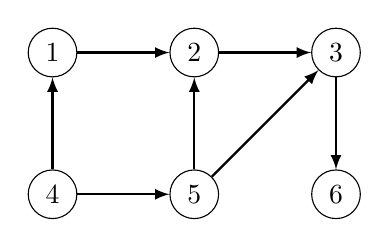
\begin{tikzpicture}[scale=0.9]
\node[draw, circle] (1) at (1,5) {$1$};
\node[draw, circle] (2) at (3,5) {$2$};
\node[draw, circle] (3) at (5,5) {$3$};
\node[draw, circle] (4) at (1,3) {$4$};
\node[draw, circle] (5) at (3,3) {$5$};
\node[draw, circle] (6) at (5,3) {$6$};

\path[draw,thick,->,>=latex] (1) -- (2);
\path[draw,thick,->,>=latex] (2) -- (3);
\path[draw,thick,->,>=latex] (4) -- (1);
\path[draw,thick,->,>=latex] (4) -- (5);
\path[draw,thick,->,>=latex] (5) -- (2);
\path[draw,thick,->,>=latex] (5) -- (3);
\path[draw,thick,->,>=latex] (3) -- (6);
\end{tikzpicture}
\end{center}
یک مرتب‌سازی توپولوژیکی
$[4,1,5,2,3,6]$ است:
\begin{center}
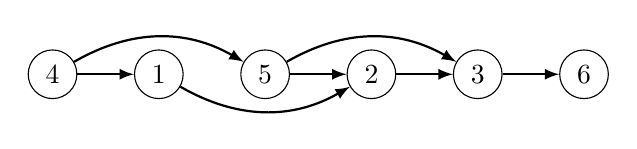
\begin{tikzpicture}[scale=0.9]
\node[draw, circle] (1) at (-6,0) {$1$};
\node[draw, circle] (2) at (-3,0) {$2$};
\node[draw, circle] (3) at (-1.5,0) {$3$};
\node[draw, circle] (4) at (-7.5,0) {$4$};
\node[draw, circle] (5) at (-4.5,0) {$5$};
\node[draw, circle] (6) at (-0,0) {$6$};

\path[draw,thick,->,>=latex] (1) edge [bend right=30] (2);
\path[draw,thick,->,>=latex] (2) -- (3);
\path[draw,thick,->,>=latex] (4) -- (1);
\path[draw,thick,->,>=latex] (4) edge [bend left=30] (5);
\path[draw,thick,->,>=latex] (5) -- (2);
\path[draw,thick,->,>=latex] (5) edge [bend left=30]  (3);
\path[draw,thick,->,>=latex] (3) -- (6);
\end{tikzpicture}
\end{center}

یک گراف بدون دور همیشه دارای مرتب‌سازی توپولوژیکی است.
با این حال، اگر گراف شامل دور باشد،
تشکیل یک مرتب‌سازی توپولوژیکی ممکن نیست،
زیرا هیچ گرهی از دور نمی‌تواند
قبل از گره‌های دیگر دور در ترتیب ظاهر شود.
مشخص می‌شود که می‌توان از جستجوی اول عمق هم برای
بررسی وجود دور در گراف جهت‌دار استفاده کرد
و هم در صورت نداشتن دور، برای ساخت یک مرتب‌سازی توپولوژیکی.

\subsubsection{الگوریتم}

ایده این است که گره‌های گراف را پیمایش کنیم
و همیشه یک جستجوی اول عمق را از گره فعلی شروع کنیم
اگر تا به حال پردازش نشده باشد.
در طول جستجوها، گره‌ها سه وضعیت ممکن دارند:

\begin{itemize}
\item وضعیت ۰: گره پردازش نشده است (سفید)
\item وضعیت ۱: گره در حال پردازش است (خاکستری روشن)
\item وضعیت ۲: گره پردازش شده است (خاکستری تیره)
\end{itemize}

در ابتدا، وضعیت هر رأس 0 است.
وقتی جستجو برای نخستین بار به رأسی می‌رسد،
وضعیت آن 1 می‌شود.
در نهایت، پس از پردازش تمام جانشین‌های رأس،
وضعیت آن 2 می‌شود.

اگر گراف دارای دور باشد، در طول جستجو
متوجه این موضوع خواهیم شد؛ چرا که دیر یا زود
به رأسی با وضعیت 1 می‌رسیم.
در این حالت، ساخت مرتب‌سازی توپولوژیکی ناممکن است.

اگر گراف فاقد دور باشد، می‌توانیم یک مرتب‌سازی
توپولوژیکی با افزودن هر رأس به یک لیست
به محض 2 شدن وضعیت آن، بسازیم.
این لیست به ترتیب معکوس، یک مرتب‌سازی توپولوژیکی است.

\subsubsection{مثال ۱}

در گراف نمونه، جستجو ابتدا از رأس 1
به رأس 6 پیش می‌رود:

\begin{center}
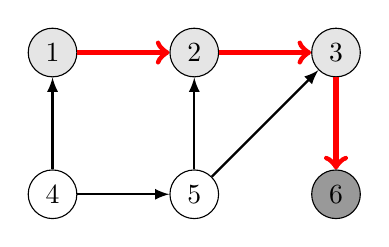
\begin{tikzpicture}[scale=0.9]
\node[draw, circle,fill=gray!20] (1) at (1,5) {$1$};
\node[draw, circle,fill=gray!20] (2) at (3,5) {$2$};
\node[draw, circle,fill=gray!20] (3) at (5,5) {$3$};
\node[draw, circle] (4) at (1,3) {$4$};
\node[draw, circle] (5) at (3,3) {$5$};
\node[draw, circle,fill=gray!80] (6) at (5,3) {$6$};

\path[draw,thick,->,>=latex] (4) -- (1);
\path[draw,thick,->,>=latex] (4) -- (5);
\path[draw,thick,->,>=latex] (5) -- (2);
\path[draw,thick,->,>=latex] (5) -- (3);
%\path[draw,thick,->,>=latex] (3) -- (6);

\path[draw=red,thick,->,line width=2pt] (1) -- (2);
\path[draw=red,thick,->,line width=2pt] (2) -- (3);
\path[draw=red,thick,->,line width=2pt] (3) -- (6);
\end{tikzpicture}
\end{center}

اکنون رأس 6 پردازش شده است، بنابراین به لیست اضافه می‌شود.
پس از آن، رأس‌های 3، 2 و 1 نیز به لیست اضافه می‌شوند:

\begin{center}
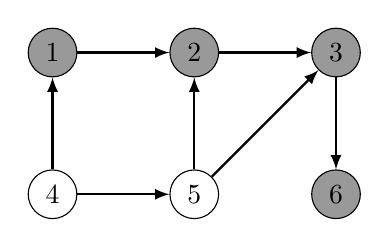
\begin{tikzpicture}[scale=0.9]
\node[draw, circle,fill=gray!80] (1) at (1,5) {$1$};
\node[draw, circle,fill=gray!80] (2) at (3,5) {$2$};
\node[draw, circle,fill=gray!80] (3) at (5,5) {$3$};
\node[draw, circle] (4) at (1,3) {$4$};
\node[draw, circle] (5) at (3,3) {$5$};
\node[draw, circle,fill=gray!80] (6) at (5,3) {$6$};

\path[draw,thick,->,>=latex] (1) -- (2);
\path[draw,thick,->,>=latex] (2) -- (3);
\path[draw,thick,->,>=latex] (4) -- (1);
\path[draw,thick,->,>=latex] (4) -- (5);
\path[draw,thick,->,>=latex] (5) -- (2);
\path[draw,thick,->,>=latex] (5) -- (3);
\path[draw,thick,->,>=latex] (3) -- (6);
\end{tikzpicture}
\end{center}

در این نقطه، لیست برابر با $[6,3,2,1]$ است.
جستجوی بعدی از رأس 4 آغاز می‌شود:

\begin{center}
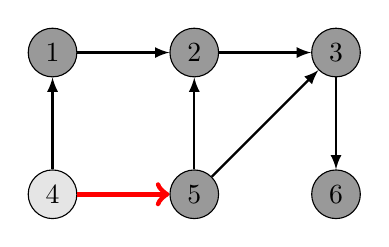
\begin{tikzpicture}[scale=0.9]
\node[draw, circle,fill=gray!80] (1) at (1,5) {$1$};
\node[draw, circle,fill=gray!80] (2) at (3,5) {$2$};
\node[draw, circle,fill=gray!80] (3) at (5,5) {$3$};
\node[draw, circle,fill=gray!20] (4) at (1,3) {$4$};
\node[draw, circle,fill=gray!80] (5) at (3,3) {$5$};
\node[draw, circle,fill=gray!80] (6) at (5,3) {$6$};

\path[draw,thick,->,>=latex] (1) -- (2);
\path[draw,thick,->,>=latex] (2) -- (3);
\path[draw,thick,->,>=latex] (4) -- (1);
%\path[draw,thick,->,>=latex] (4) -- (5);
\path[draw,thick,->,>=latex] (5) -- (2);
\path[draw,thick,->,>=latex] (5) -- (3);
\path[draw,thick,->,>=latex] (3) -- (6);

\path[draw=red,thick,->,line width=2pt] (4) -- (5);
\end{tikzpicture}
\end{center}

بنابراین لیست نهایی $[6,3,2,1,5,4]$ است.
همه گره‌ها پردازش شدند، پس مرتب‌سازی توپولوژیک پیدا شد.
مرتب‌سازی توپولوژیک معکوس این لیست است:
$[4,5,1,2,3,6]$:

\begin{center}
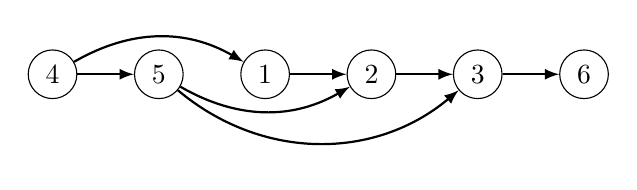
\begin{tikzpicture}[scale=0.9]
\node[draw, circle] (1) at (3,0) {$1$};
\node[draw, circle] (2) at (4.5,0) {$2$};
\node[draw, circle] (3) at (6,0) {$3$};
\node[draw, circle] (4) at (0,0) {$4$};
\node[draw, circle] (5) at (1.5,0) {$5$};
\node[draw, circle] (6) at (7.5,0) {$6$};

\path[draw,thick,->,>=latex] (1) -- (2);
\path[draw,thick,->,>=latex] (2) -- (3);
\path[draw,thick,->,>=latex] (4) edge [bend left=30] (1);
\path[draw,thick,->,>=latex] (4) -- (5);
\path[draw,thick,->,>=latex] (5) edge [bend right=30] (2);
\path[draw,thick,->,>=latex] (5) edge [bend right=40] (3);
\path[draw,thick,->,>=latex] (3) -- (6);
\end{tikzpicture}
\end{center}

مرتب‌سازی توپولوژیک یکتا نیست.
گراف می‌تواند چند مرتب‌سازی توپولوژیک داشته باشد.

\subsubsection{مثال ۲}

گرافی بدون مرتب‌سازی توپولوژیک بررسی می‌شود،
چون گراف دور دارد:

\begin{center}
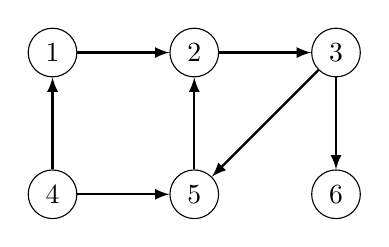
\begin{tikzpicture}[scale=0.9]
\node[draw, circle] (1) at (1,5) {$1$};
\node[draw, circle] (2) at (3,5) {$2$};
\node[draw, circle] (3) at (5,5) {$3$};
\node[draw, circle] (4) at (1,3) {$4$};
\node[draw, circle] (5) at (3,3) {$5$};
\node[draw, circle] (6) at (5,3) {$6$};

\path[draw,thick,->,>=latex] (1) -- (2);
\path[draw,thick,->,>=latex] (2) -- (3);
\path[draw,thick,->,>=latex] (4) -- (1);
\path[draw,thick,->,>=latex] (4) -- (5);
\path[draw,thick,->,>=latex] (5) -- (2);
\path[draw,thick,->,>=latex] (3) -- (5);
\path[draw,thick,->,>=latex] (3) -- (6);
\end{tikzpicture}
\end{center}
روند جستجو:
\begin{center}
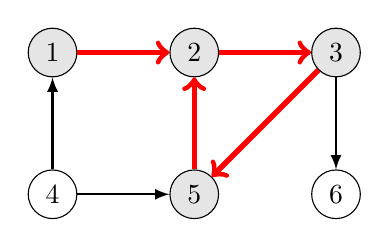
\begin{tikzpicture}[scale=0.9]
\node[draw, circle,fill=gray!20] (1) at (1,5) {$1$};
\node[draw, circle,fill=gray!20] (2) at (3,5) {$2$};
\node[draw, circle,fill=gray!20] (3) at (5,5) {$3$};
\node[draw, circle] (4) at (1,3) {$4$};
\node[draw, circle,fill=gray!20] (5) at (3,3) {$5$};
\node[draw, circle] (6) at (5,3) {$6$};

\path[draw,thick,->,>=latex] (4) -- (1);
\path[draw,thick,->,>=latex] (4) -- (5);
\path[draw,thick,->,>=latex] (3) -- (6);

\path[draw=red,thick,->,line width=2pt] (1) -- (2);
\path[draw=red,thick,->,line width=2pt] (2) -- (3);
\path[draw=red,thick,->,line width=2pt] (3) -- (5);
\path[draw=red,thick,->,line width=2pt] (5) -- (2);
\end{tikzpicture}
\end{center}
جستجو به گره 2 با وضعیت 1 می‌رسد.
یعنی گراف دور دارد.
در این مثال، دور برابر است با:
$2 \rightarrow 3 \rightarrow 5 \rightarrow 2$.

\section{برنامه‌نویسی پویا}

اگر گراف جهت‌دار بدون دور باشد،
برنامه‌نویسی پویا روی آن قابل اعمال است.
مسائل زیر برای مسیرهای بین گره آغازین
و پایانی سریع حل می‌شوند:

\begin{itemize}
\item چند مسیر متمایز وجود دارد؟
\item کوتاه‌ترین/طولانی‌ترین مسیر کدام است؟
\item کمینه/بیشینه تعداد یال‌ها در یک مسیر چقدر است؟
\item کدام رأس‌ها قطعاً در هر مسیری ظاهر می‌شوند؟
\end{itemize}

\subsubsection{شمارش تعداد مسیرها}

به عنوان مثال، بیایید تعداد مسیرها از رأس ۱ به رأس ۶ را در گراف زیر محاسبه کنیم:

\begin{center}
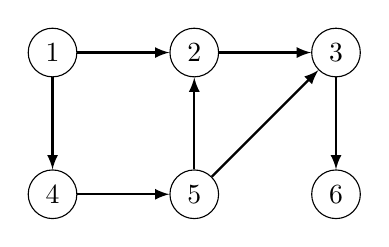
\begin{tikzpicture}[scale=0.9]
\node[draw, circle] (1) at (1,5) {$1$};
\node[draw, circle] (2) at (3,5) {$2$};
\node[draw, circle] (3) at (5,5) {$3$};
\node[draw, circle] (4) at (1,3) {$4$};
\node[draw, circle] (5) at (3,3) {$5$};
\node[draw, circle] (6) at (5,3) {$6$};

\path[draw,thick,->,>=latex] (1) -- (2);
\path[draw,thick,->,>=latex] (2) -- (3);
\path[draw,thick,->,>=latex] (1) -- (4);
\path[draw,thick,->,>=latex] (4) -- (5);
\path[draw,thick,->,>=latex] (5) -- (2);
\path[draw,thick,->,>=latex] (5) -- (3);
\path[draw,thick,->,>=latex] (3) -- (6);
\end{tikzpicture}
\end{center}
در مجموع سه مسیر این‌چنینی وجود دارد:
\begin{itemize}
\item $1 \rightarrow 2 \rightarrow 3 \rightarrow 6$
\item $1 \rightarrow 4 \rightarrow 5 \rightarrow 2 \rightarrow 3 \rightarrow 6$
\item $1 \rightarrow 4 \rightarrow 5 \rightarrow 3 \rightarrow 6$
\end{itemize}

فرض کنید $\texttt{paths}(x)$ بیانگر تعداد مسیرها از رأس ۱ به رأس $x$ باشد.
به عنوان حالت پایه، $\texttt{paths}(1)=1$.
سپس، برای محاسبه سایر مقادیر $\texttt{paths}(x)$، می‌توان از رابطه بازگشتی زیر استفاده کرد:
\[\texttt{paths}(x) = \texttt{paths}(a_1)+\texttt{paths}(a_2)+\cdots+\texttt{paths}(a_k)\]
که در آن $a_1,a_2,\ldots,a_k$ رأس‌هایی هستند که از آن‌ها یالی به $x$ وجود دارد.
از آنجا که گراف بدون دور است، مقادیر $\texttt{paths}(x)$ را می‌توان به ترتیب مرتب‌سازی توپولوژیکی محاسبه کرد.
یک مرتب‌سازی توپولوژیکی برای گراف بالا به صورت زیر است:
\begin{center}
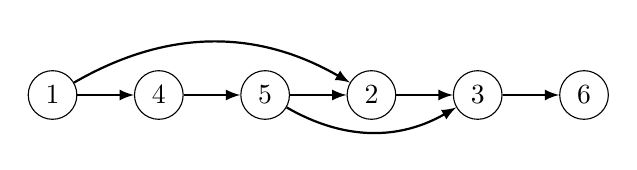
\begin{tikzpicture}[scale=0.9]
\node[draw, circle] (1) at (0,0) {$1$};
\node[draw, circle] (2) at (4.5,0) {$2$};
\node[draw, circle] (3) at (6,0) {$3$};
\node[draw, circle] (4) at (1.5,0) {$4$};
\node[draw, circle] (5) at (3,0) {$5$};
\node[draw, circle] (6) at (7.5,0) {$6$};

\path[draw,thick,->,>=latex] (1) edge [bend left=30] (2);
\path[draw,thick,->,>=latex] (2) -- (3);
\path[draw,thick,->,>=latex] (1) -- (4);
\path[draw,thick,->,>=latex] (4) -- (5);
\path[draw,thick,->,>=latex] (5) -- (2);
\path[draw,thick,->,>=latex] (5) edge [bend right=30] (3);
\path[draw,thick,->,>=latex] (3) -- (6);
\end{tikzpicture}
\end{center}
بنابراین، تعداد مسیرها به شرح زیر است:
\begin{center}
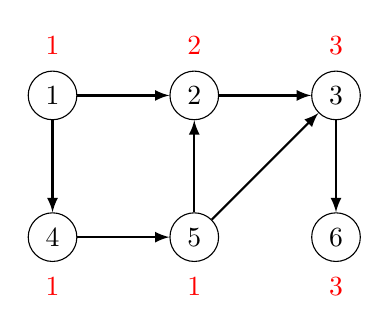
\begin{tikzpicture}[scale=0.9]
\node[draw, circle] (1) at (1,5) {$1$};
\node[draw, circle] (2) at (3,5) {$2$};
\node[draw, circle] (3) at (5,5) {$3$};
\node[draw, circle] (4) at (1,3) {$4$};
\node[draw, circle] (5) at (3,3) {$5$};
\node[draw, circle] (6) at (5,3) {$6$};

\path[draw,thick,->,>=latex] (1) -- (2);
\path[draw,thick,->,>=latex] (2) -- (3);
\path[draw,thick,->,>=latex] (1) -- (4);
\path[draw,thick,->,>=latex] (4) -- (5);
\path[draw,thick,->,>=latex] (5) -- (2);
\path[draw,thick,->,>=latex] (5) -- (3);
\path[draw,thick,->,>=latex] (3) -- (6);

\node[color=red] at (1,2.3) {$1$};
\node[color=red] at (3,2.3) {$1$};
\node[color=red] at (5,2.3) {$3$};
\node[color=red] at (1,5.7) {$1$};
\node[color=red] at (3,5.7) {$2$};
\node[color=red] at (5,5.7) {$3$};
\end{tikzpicture}
\end{center}

برای مثال، جهت محاسبه مقدار $\texttt{paths}(3)$،
می‌توان از فرمول $\texttt{paths}(2)+\texttt{paths}(5)$ استفاده کرد،
زیرا یال‌هایی از گره‌های ۲ و ۵
به گره ۳ وجود دارد.
از آنجا که $\texttt{paths}(2)=2$ و $\texttt{paths}(5)=1$ است، نتیجه می‌گیریم $\texttt{paths}(3)=3$.

\subsubsection{گسترش الگوریتم دایکسترا}

\index{الگوریتم دایکسترا}

یک نتیجه جانبی الگوریتم دایکسترا، گراف جهت‌دار بدون دور است
که برای هر گره از گراف اصلی،
مسیرهای ممکن برای رسیدن به آن گره با استفاده از کوتاه‌ترین مسیر
از گره مبدا را مشخص می‌کند.
می‌توان برنامه‌نویسی پویا را روی این گراف اعمال کرد.
به عنوان مثال، در گراف
\begin{center}
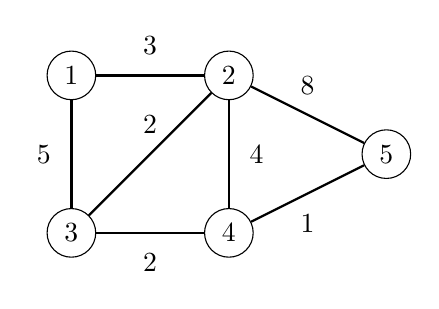
\begin{tikzpicture}
\node[draw, circle] (1) at (0,0) {$1$};
\node[draw, circle] (2) at (2,0) {$2$};
\node[draw, circle] (3) at (0,-2) {$3$};
\node[draw, circle] (4) at (2,-2) {$4$};
\node[draw, circle] (5) at (4,-1) {$5$};

\path[draw,thick,-] (1) -- node[font=\small,label=above:3] {} (2);
\path[draw,thick,-] (1) -- node[font=\small,label=left:5] {} (3);
\path[draw,thick,-] (2) -- node[font=\small,label=right:4] {} (4);
\path[draw,thick,-] (2) -- node[font=\small,label=above:8] {} (5);
\path[draw,thick,-] (3) -- node[font=\small,label=below:2] {} (4);
\path[draw,thick,-] (4) -- node[font=\small,label=below:1] {} (5);
\path[draw,thick,-] (2) -- node[font=\small,label=above:2] {} (3);
\end{tikzpicture}
\end{center}
کوتاه‌ترین مسیرها از گره ۱ ممکن است از یال‌های زیر استفاده کنند:
\begin{center}
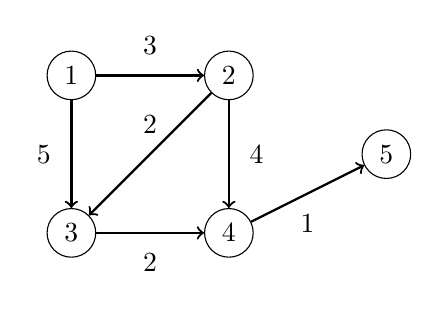
\begin{tikzpicture}
\node[draw, circle] (1) at (0,0) {$1$};
\node[draw, circle] (2) at (2,0) {$2$};
\node[draw, circle] (3) at (0,-2) {$3$};
\node[draw, circle] (4) at (2,-2) {$4$};
\node[draw, circle] (5) at (4,-1) {$5$};

\path[draw,thick,->] (1) -- node[font=\small,label=above:3] {} (2);
\path[draw,thick,->] (1) -- node[font=\small,label=left:5] {} (3);
\path[draw,thick,->] (2) -- node[font=\small,label=right:4] {} (4);
\path[draw,thick,->] (3) -- node[font=\small,label=below:2] {} (4);
\path[draw,thick,->] (4) -- node[font=\small,label=below:1] {} (5);
\path[draw,thick,->] (2) -- node[font=\small,label=above:2] {} (3);
\end{tikzpicture}
\end{center}

اکنون می‌توانیم به عنوان نمونه، تعداد
کوتاه‌ترین مسیرها از گره ۱ به گره ۵ را
با استفاده از برنامه‌نویسی پویا محاسبه کنیم:
\begin{center}
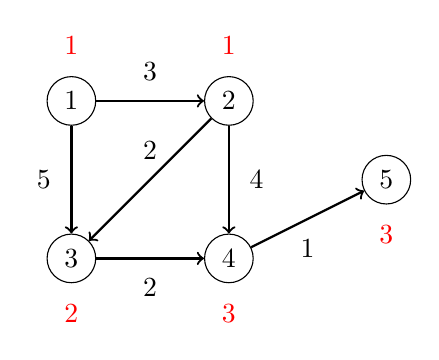
\begin{tikzpicture}
\node[draw, circle] (1) at (0,0) {$1$};
\node[draw, circle] (2) at (2,0) {$2$};
\node[draw, circle] (3) at (0,-2) {$3$};
\node[draw, circle] (4) at (2,-2) {$4$};
\node[draw, circle] (5) at (4,-1) {$5$};

\path[draw,thick,->] (1) -- node[font=\small,label=above:3] {} (2);
\path[draw,thick,->] (1) -- node[font=\small,label=left:5] {} (3);
\path[draw,thick,->] (2) -- node[font=\small,label=right:4] {} (4);
\path[draw,thick,->] (3) -- node[font=\small,label=below:2] {} (4);
\path[draw,thick,->] (4) -- node[font=\small,label=below:1] {} (5);
\path[draw,thick,->] (2) -- node[font=\small,label=above:2] {} (3);

\node[color=red] at (0,0.7) {$1$};
\node[color=red] at (2,0.7) {$1$};
\node[color=red] at (0,-2.7) {$2$};
\node[color=red] at (2,-2.7) {$3$};
\node[color=red] at (4,-1.7) {$3$};
\end{tikzpicture}
\end{center}

\subsubsection{نمایش مسائل به صورت گراف}

در واقع، هر مسئله برنامه‌نویسی پویا
می‌تواند به صورت یک گراف جهت‌دار بدون دور نمایش داده شود.
در چنین گرافی، هر گره متناظر با یک وضعیت برنامه‌نویسی پویا است
و یال‌ها نشان می‌دهند که وضعیت‌ها چگونه به یکدیگر وابسته‌اند.

به عنوان مثال، مسئله ساختن مقدار پول $n$
با استفاده از سکه‌های
$\{c_1,c_2,\ldots,c_k\}$
را در نظر بگیرید.
در این مسئله، می‌توان گرافی ساخت که در آن
هر گره متناظر با یک مقدار پول است،
و یال‌ها نحوه انتخاب سکه‌ها را نشان می‌دهند.
برای نمونه، به ازای سکه‌های $\{1,3,4\}$ و $n=6$،
گراف به صورت زیر است:
\begin{center}
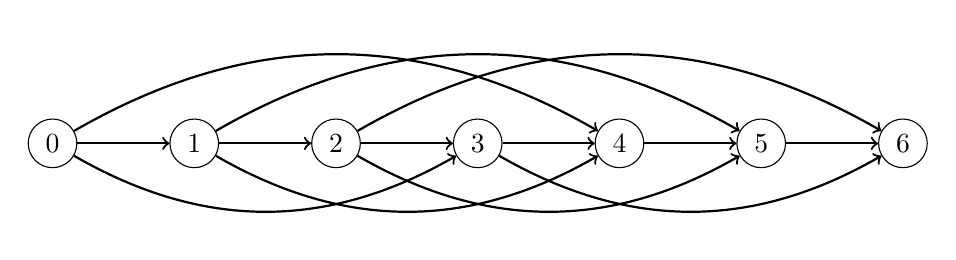
\begin{tikzpicture}[scale=0.9]
\node[draw, circle] (0) at (0,0) {$0$};
\node[draw, circle] (1) at (2,0) {$1$};
\node[draw, circle] (2) at (4,0) {$2$};
\node[draw, circle] (3) at (6,0) {$3$};
\node[draw, circle] (4) at (8,0) {$4$};
\node[draw, circle] (5) at (10,0) {$5$};
\node[draw, circle] (6) at (12,0) {$6$};

\path[draw,thick,->] (0) -- (1);
\path[draw,thick,->] (1) -- (2);
\path[draw,thick,->] (2) -- (3);
\path[draw,thick,->] (3) -- (4);
\path[draw,thick,->] (4) -- (5);
\path[draw,thick,->] (5) -- (6);

\path[draw,thick,->] (0) edge [bend right=30] (3);
\path[draw,thick,->] (1) edge [bend right=30] (4);
\path[draw,thick,->] (2) edge [bend right=30] (5);
\path[draw,thick,->] (3) edge [bend right=30] (6);

\path[draw,thick,->] (0) edge [bend left=30] (4);
\path[draw,thick,->] (1) edge [bend left=30] (5);
\path[draw,thick,->] (2) edge [bend left=30] (6);
\end{tikzpicture}
\end{center}

با استفاده از این نمایش،
کوتاه‌ترین مسیر از گره 0 به گره $n$
متناظر با پاسخی با کمترین تعداد سکه است،
و تعداد کل مسیرها از گره 0 به گره $n$
برابر با تعداد کل راه‌حل‌ها است.

\section{مسیرهای جانشین}

\index{گراف جانشین}
\index{گراف تابعی}

در ادامه این فصل،
بر روی \key{گراف‌های جانشین} تمرکز خواهیم کرد.
در این گراف‌ها،
درجه خروجی هر گره ۱ است، یعنی
دقیقاً یک یال از هر گره شروع می‌شود.
یک گراف جانشین شامل یک یا چند
مؤلفه است که هر کدام شامل
یک دور و مسیرهایی است که به آن منتهی می‌شوند.

گراف‌های جانشین گاهی اوقات
\key{گراف‌های تابعی} نامیده می‌شوند.
دلیل این نام‌گذاری این است که هر گراف جانشین
متناظر با تابعی است که
یال‌های گراف را تعریف می‌کند.
پارامتر ورودی تابع یک گره از گراف است،
و خروجی تابع گره جانشین آن خواهد بود.

برای مثال، تابع
\begin{center}
\begin{tabular}{r|rrrrrrrrr}
$x$ & 1 & 2 & 3 & 4 & 5 & 6 & 7 & 8 & 9 \\
\hline
$\texttt{succ}(x)$ & 3 & 5 & 7 & 6 & 2 & 2 & 1 & 6 & 3 \\
\end{tabular}
\end{center}
گراف زیر را تعریف می‌کند:
\begin{center}
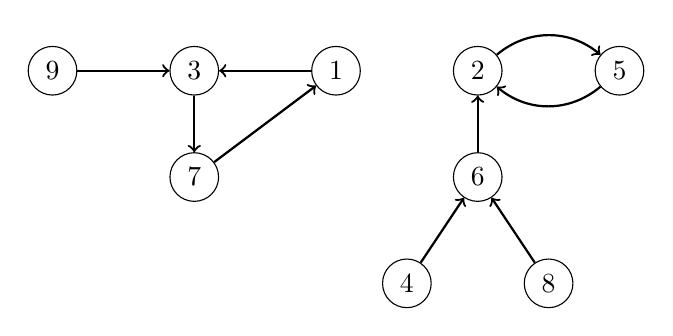
\begin{tikzpicture}[scale=0.9]
\node[draw, circle] (1) at (0,0) {$1$};
\node[draw, circle] (2) at (2,0) {$2$};
\node[draw, circle] (3) at (-2,0) {$3$};
\node[draw, circle] (4) at (1,-3) {$4$};
\node[draw, circle] (5) at (4,0) {$5$};
\node[draw, circle] (6) at (2,-1.5) {$6$};
\node[draw, circle] (7) at (-2,-1.5) {$7$};
\node[draw, circle] (8) at (3,-3) {$8$};
\node[draw, circle] (9) at (-4,0) {$9$};

\path[draw,thick,->] (1) -- (3);
\path[draw,thick,->] (2)  edge [bend left=40] (5);
\path[draw,thick,->] (3) -- (7);
\path[draw,thick,->] (4) -- (6);
\path[draw,thick,->] (5)  edge [bend left=40] (2);
\path[draw,thick,->] (6) -- (2);
\path[draw,thick,->] (7) -- (1);
\path[draw,thick,->] (8) -- (6);
\path[draw,thick,->] (9) -- (3);
\end{tikzpicture}
\end{center}

از آنجا که هر راس در گراف جانشین دارای یک جانشین یکتا است، می‌توانیم تابع $\texttt{succ}(x,k)$ را نیز تعریف کنیم که راسی را مشخص می‌کند که با شروع از راس $x$ و پیمودن $k$ گام به سمت جلو به آن می‌رسیم.
برای نمونه، در گراف بالا $\texttt{succ}(4,6)=2$ است، زیرا با طی کردن ۶ گام از راس ۴ به راس ۲ می‌رسیم:

\begin{center}
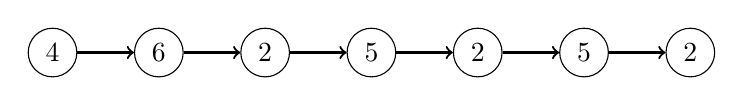
\begin{tikzpicture}[scale=0.9]
\node[draw, circle] (1) at (0,0) {$4$};
\node[draw, circle] (2) at (1.5,0) {$6$};
\node[draw, circle] (3) at (3,0) {$2$};
\node[draw, circle] (4) at (4.5,0) {$5$};
\node[draw, circle] (5) at (6,0) {$2$};
\node[draw, circle] (6) at (7.5,0) {$5$};
\node[draw, circle] (7) at (9,0) {$2$};

\path[draw,thick,->] (1) -- (2);
\path[draw,thick,->] (2) -- (3);
\path[draw,thick,->] (3) -- (4);
\path[draw,thick,->] (4) -- (5);
\path[draw,thick,->] (5) -- (6);
\path[draw,thick,->] (6) -- (7);
\end{tikzpicture}
\end{center}

یک روش سرراست برای محاسبه مقدار $\texttt{succ}(x,k)$ شروع از راس $x$ و پیمودن $k$ گام رو به جلو است که به زمان $O(k)$ نیاز دارد.
با این حال، با استفاده از پیش‌پردازش، هر مقدار از $\texttt{succ}(x,k)$ تنها در زمان $O(\log k)$ قابل محاسبه است.

ایده کار، پیش‌محاسبه تمام مقادیر $\texttt{succ}(x,k)$ است که در آن $k$ توانی از دو و حداکثر برابر با $u$ باشد؛ به طوری که $u$ حداکثر تعداد گام‌هایی است که پیمایش خواهیم کرد.
این کار با بازگشت زیر به صورت کارا انجام‌پذیر است:

\begin{equation*}
    \texttt{succ}(x,k) = \begin{cases}
               \texttt{succ}(x)              & k = 1\\
               \texttt{succ}(\texttt{succ}(x,k/2),k/2)   & k > 1\\
           \end{cases}
\end{equation*}

پیش‌محاسبه مقادیر، زمان $O(n \log u)$ می‌برد، زیرا برای هر راس $O(\log u)$ مقدار محاسبه می‌شود.
در گراف بالا، مقادیر اولیه به صورت زیر هستند:

\begin{center}
\begin{tabular}{r|rrrrrrrrr}
$x$ & 1 & 2 & 3 & 4 & 5 & 6 & 7 & 8 & 9 \\
\hline
$\texttt{succ}(x,1)$ & 3 & 5 & 7 & 6 & 2 & 2 & 1 & 6 & 3 \\
$\texttt{succ}(x,2)$ & 7 & 2 & 1 & 2 & 5 & 5 & 3 & 2 & 7 \\
$\texttt{succ}(x,4)$ & 3 & 2 & 7 & 2 & 5 & 5 & 1 & 2 & 3 \\
$\texttt{succ}(x,8)$ & 7 & 2 & 1 & 2 & 5 & 5 & 3 & 2 & 7 \\
$\cdots$ \\
\end{tabular}
\end{center}

پس از این، هر مقدار $\texttt{succ}(x,k)$ را می‌توان با نمایش تعداد گام‌های $k$ به صورت مجموع توان‌های دو محاسبه کرد.
به عنوان مثال، برای محاسبه مقدار $\texttt{succ}(x,11)$،
ابتدا نمایش $11=8+2+1$ را تشکیل می‌دهیم.
با استفاده از آن،
\[\texttt{succ}(x,11)=\texttt{succ}(\texttt{succ}(\texttt{succ}(x,8),2),1).\]
به عنوان مثال، در گراف قبلی
\[\texttt{succ}(4,11)=\texttt{succ}(\texttt{succ}(\texttt{succ}(4,8),2),1)=5.\]

چنین نمایشی همیشه شامل $O(\log k)$ بخش است، بنابراین محاسبه مقدار $\texttt{succ}(x,k)$
زمان $O(\log k)$ می‌برد.

\section{تشخیص دور}

\index{cycle}
\index{cycle detection}

یک گراف جانشین را در نظر بگیرید که فقط شامل یک مسیر منتهی به دور است.
می‌توان پرسش‌های زیر را مطرح کرد:
اگر پیمایش را از راس آغازین شروع کنیم،
اولین راس در دور کدام است
و دور شامل چند راس است؟

به عنوان مثال، در گراف

\begin{center}
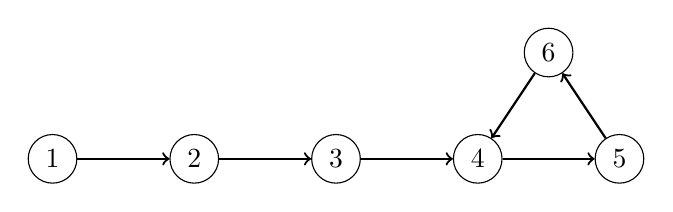
\begin{tikzpicture}[scale=0.9]
\node[draw, circle] (5) at (0,0) {$5$};
\node[draw, circle] (4) at (-2,0) {$4$};
\node[draw, circle] (6) at (-1,1.5) {$6$};
\node[draw, circle] (3) at (-4,0) {$3$};
\node[draw, circle] (2) at (-6,0) {$2$};
\node[draw, circle] (1) at (-8,0) {$1$};

\path[draw,thick,->] (1) -- (2);
\path[draw,thick,->] (2) -- (3);
\path[draw,thick,->] (3) -- (4);
\path[draw,thick,->] (4) -- (5);
\path[draw,thick,->] (5) -- (6);
\path[draw,thick,->] (6) -- (4);
\end{tikzpicture}
\end{center}
پیمایش را از راس ۱ شروع می‌کنیم،
اولین راسی که متعلق به دور است راس ۴ بوده و دور متشکل از سه راس (۴، ۵ و ۶) است.

یک روش ساده برای تشخیص دور، پیمایش گراف و ردگیری همه راس‌های دیده‌شده است.
به محض این‌که راسی برای بار دوم دیده شود، می‌توان نتیجه گرفت
که این راس، اولین راس در دور است.
این روش در زمان $O(n)$ اجرا می‌شود و از $O(n)$ حافظه استفاده می‌کند.

با این حال، الگوریتم‌های بهتری برای تشخیص دور وجود دارند.
پیچیدگی زمانی چنین الگوریتم‌هایی هنوز $O(n)$ است،
اما تنها از $O(1)$ حافظه استفاده می‌کنند.
این یک بهینه‌سازی مهم برای مقادیر بزرگ $n$ است.
در ادامه به الگوریتم فلوید می‌پردازیم که این ویژگی‌ها را داراست.

\subsubsection{الگوریتم فلوید}

\index{Floyd's algorithm}

\key{الگوریتم فلوید}\footnote{ایده الگوریتم در \cite{knu982} ذکر شده و به آر. دبلیو. فلوید نسبت داده شده؛ ولی معلوم نیست فلوید واقعا کشف کرد یا نه.} با دو اشاره‌گر $a$ و $b$ در گراف جلو می‌رود.
هر دو اشاره‌گر از گره $x$، گره شروع گراف، آغاز می‌کنند.
سپس هر نوبت، اشاره‌گر $a$ یک گام و اشاره‌گر $b$ دو گام جلو می‌روند.
فرآیند تا زمان برخورد اشاره‌گرها ادامه دارد:
\begin{lstlisting}
a = succ(x);
b = succ(succ(x));
while (a != b) {
    a = succ(a);
    b = succ(succ(b));
}
\end{lstlisting}

این نقطه، اشاره‌گر $a$ به اندازه $k$ گام و اشاره‌گر $b$ به اندازه $2k$ گام رفته‌اند، پس طول دور شمارنده $k$ است.
بنابراین اولین گره دور با بردن اشاره‌گر $a$ به گره $x$ و حرکت گام‌به‌گام اشاره‌گرها تا برخورد دوباره پیدا می‌شود.
\begin{lstlisting}
a = x;
while (a != b) {
    a = succ(a);
    b = succ(b);
}
first = a;
\end{lstlisting}

سپس طول دور این‌طور حساب می‌شود:
\begin{lstlisting}
b = succ(a);
length = 1;
while (a != b) {
    b = succ(b);
    length++;
}
\end{lstlisting}